%(BEGIN_QUESTION)
% Copyright 2009, Tony R. Kuphaldt, released under the Creative Commons Attribution License (v 1.0)
% This means you may do almost anything with this work of mine, so long as you give me proper credit

Vi har et rør som det strømmer olje med en strømningsrate på 120 m³/h og en temperatur på 50°C. Begge seksjonene er etter schedule 40.  Den første delen av røret har dimensjon DN200 (ID=202.74mm) og den andre delen har dimensjon DN65 (ID=62.68mm)

$$\includegraphics[width=15.5cm]{i04033x01.eps}$$

Regn ut hastigheten for fluidet i røret h hver av seksjonene. Regn også ut den volumentriske strømningsraten i \textit{gallons per minute} (GPM). 


\vskip 10pt

I hvilken seksjon av røret har oljestrømmen høyest reynolds nummer?

\vskip 20pt \vbox{\hrule \hbox{\strut \vrule{} {\bf Suggestions for Socratic discussion} \vrule} \hrule}

\begin{itemize}
\item{} This question is a good application of the {\it Law of Continuity}, but this law is really nothing more than an expression of a more fundamental law in physics.  What is this more fundamental law, and what does it tell us about flow through a pipe?
\item{} Once we know the fluid velocity in one section of the pipe, show how we may calculate the velocity in the other section of the pipe using nothing but a ratio of pipe diameters ($7.981 \over 2.469$), rather than re-calculate the continuity formula again ($v = {Q \over A}$).
\item{} Where along this pipe will individual fluid molecules possess the greatest kinetic energy?
\end{itemize}

Schedule 40 Pipe 8 Inch (DN200 mm)\\
Standard : ANSI/ASME B36.10(Steel Pipe)\\
– Size : NPS 8 Inch\\
– Size : DN200 mm\\
– Inside Dimeter(Pipe ID) : 202.74 mm\\
– Outside Dimeter(Pipe OD) : 219.1 mm\\
– Pipe Wall Thickness : 8.18 mm\\
– Pipe Weight : 42.55 Kilogram per meter (kg/m)\\
– Pipe Weight Including Water : 74.81 Kilogram per meter (kg/m)\\
*NPS = Nominal pipe size(inch) / DN = Diameter nominal(mm)\\
\\\\
Schedule 40 Pipe 2 1/2 Inch (DN65 mm)\\
Standard : ANSI/ASME B36.10(Steel Pipe)\\
– Size : NPS 2 1/2 Inch\\
– Size : DN65 mm\\
– Inside Dimeter(Pipe ID) : 62.68 mm\\
– Outside Dimeter(Pipe OD) : 73 mm\\
– Pipe Wall Thickness : 5.16 mm\\
– Pipe Weight : 8.63 Kilogram per meter (kg/m)\\
– Pipe Weight Including Water : 11.71 Kilogram per meter (kg/m)\\
*NPS = Nominal pipe size(inch) / DN = Diameter nominal(mm)\\
\underbar{file i04033}
%(END_QUESTION)





%(BEGIN_ANSWER)

\noindent
{\bf Partial answer:}

\vskip 10pt

$\overline{v}$ through the 8-inch pipe = 201.49 feet per minute.

%(END_ANSWER)





%(BEGIN_NOTES)

$$Q = A \overline{v}$$

Average flow velocity through the 8 inch pipe:

$$\overline{v} = {Q \over A} = {70 \hbox{ ft}^3/\hbox{min} \over 0.3474 \hbox{ ft}^2} = 201.49 \hbox{ ft/min}$$

\vskip 10pt

Average flow velocity through the 2.5 inch pipe:

$$\overline{v} = {Q \over A} = {70 \hbox{ ft}^3/\hbox{min} \over 0.03325 \hbox{ ft}^2} = 2105.4 \hbox{ ft/min}$$

\vskip 10pt

$$\left({70 \hbox{ ft}^3 \over \hbox{min}}\right) \left({1728 \hbox{ in}^3 \over \hbox{ft}^3}\right) \left({1 \hbox{ gal} \over 231 \hbox{ in}^3} \right) = 523.64 \hbox{ GPM}$$

\vskip 10pt

The oil's temperature of 113 degrees F is extraneous information, included for the purpose of challenging students to identify whether or not information is relevant to solving a particular problem.








\vfil \eject

\noindent
{\bf Prep Quiz:}

Calculate the velocity of the fluid through the narrow section of pipe, if the velocity through the wide section is 7 feet per second:

$$\includegraphics[width=15.5cm]{i04033x02.eps}$$

\begin{itemize}
\item{} 2.33 ft/s
\vskip 5pt 
\item{} 7 ft/s
\vskip 5pt 
\item{} 99 ft/s
\vskip 5pt 
\item{} 21 ft/s
\vskip 5pt 
\item{} 9 ft/s 
\vskip 5pt 
\item{} 63 ft/s
\end{itemize}

\vfil \eject

\noindent
{\bf Prep Quiz:}

Calculate the velocity of the fluid through the narrow section of pipe, if the velocity through the wide section is 11 feet per second:

$$\includegraphics[width=15.5cm]{i04033x02.eps}$$

\begin{itemize}
\item{} 11 ft/s
\vskip 5pt 
\item{} 1.22 ft/s
\vskip 5pt 
\item{} 6 ft/s
\vskip 5pt 
\item{} 99 ft/s
\vskip 5pt 
\item{} 9 ft/s 
\vskip 5pt 
\item{} 63 ft/s
\end{itemize}


%INDEX% Physics, dynamic fluids: continuity equation

%(END_NOTES)


